\documentclass[12pt]{article}
\usepackage{amsmath,amssymb,multirow, float, amsthm}
\usepackage{graphicx,psfrag,epsf}
\usepackage{enumerate}
\usepackage{natbib}
\usepackage{url} % not crucial - just used below for the URL

%\pdfminorversion=4
% NOTE: To produce blinded version, replace "0" with "1" below.
\newcommand{\blind}{0}

% DON'T change margins - should be 1 inch all around.
\addtolength{\oddsidemargin}{-.5in}%
\addtolength{\evensidemargin}{-.5in}%
\addtolength{\textwidth}{1in}%
\addtolength{\textheight}{1.3in}%
\addtolength{\topmargin}{-.8in}%
\newtheorem{theorem}{Theorem}

\begin{document}

%\bibliographystyle{natbib}

\def\spacingset#1{\renewcommand{\baselinestretch}%
{#1}\small\normalsize} \spacingset{1}


%%%%%%%%%%%%%%%%%%%%%%%%%%%%%%%%%%%%%%%%%%%%%%%%%%%%%%%%%%%%%%%%%%%%%%%%%%%%%%

\if0\blind
{
  \title{\bf Backtesting CoVaR}
  \author{Author 1\\
    Department of YYY, University of XXX\\
    and \\
    Author 2 \\
    Department of ZZZ, University of WWW}
  \maketitle
} \fi

\if1\blind
{
  \bigskip
  \bigskip
  \bigskip
  \begin{center}
    {\LARGE\bf Backtesting (Delta-)CoVaR}
\end{center}
  \medskip
} \fi

\bigskip
\begin{abstract}
%In this paper we propose a new backtesting method for Conditional Value at Risk ($CoVaR$), a systemic risk measure introduced by \citet{adrian}. Instead of testing the subset of $CoVaR$ predictions in which the condition is satisfied (the approach used in previous research), we predict the $CoVaR$ as a function of its condition, and evaluate the predicted $CoVaR$ at the realisation of this condition. This allows us to perform tests on the full set of $CoVaR$ predictions. In our Monte Carlo study we show that our test is useful in a realistic setting and that it outperforms previous $CoVaR$ backtesting methods. Finally, we apply our test to real world data and use it to compare the performance of different $CoVaR$ prediction methods.
We propose a new backtesting method for Delta-CoVaR. This measure of systemic risk is defined as the increase in Value of Risk of a financial institution when the financial system is in distress (i.e., when it violates its own VaR) compared to a non-distress state (when its return is at the median). By relying on a conditional version of the probability integral transform, we are able to exploit the entire sample of CoVaR predictions, rather than just the periods in which the system is in distress. A Monte Carlo study demonstrates that the new test has dramatically increased power vis-a-vis existing tests. An empirical application demonstrates the use of the test in a real-world scenario.
\end{abstract}
{\it Keywords:}  Backtest; CoVaR; Systemic risk.
\vfill

\newpage
\spacingset{1.45} % DON'T change the spacing!




%%% 1 INTRODUCTION %%%

\section{Introduction}


Since the financial crisis, there has been a lot of attention for systemic risk, the risk that one institution in financial distress can contaminate the entire financial system. Federal Reserve Governor Daniel Tarullo formulated systemic importance in a 2009 testimony before the Senate Banking, Housing, and Urban Affairs Committee as follows:\footnote{Source: https://www.federalreserve.gov/newsevents/testimony/tarullo20090723a.htm}

\textit{``Financial institutions are systemically important if the failure of the firm to meet its obligations to creditors and customers would have significant adverse consequences for the financial system and the broader economy."}

The most widely used risk measure in finance was (and still is) the Value at Risk ($VaR$), which is defined as the maximum return loss of a financial institution within a certain probability. The $VaR$ focuses on one financial institution in isolation and does not capture its risk contribution to the financial system. Therefore, there has been a lot of interest in risk measures which take the interaction between financial institutions into account. Systemic risk measures aim to capture the amount of risk in the financial system that can be attributed to a financial institution.

Several systemic risk measures have been developed. \citet{billio} use the time variation in the number of principal components necessary to explain a certain fraction of the volatility of the return of the financial system, to determine the time variation in the level of interconnectedness between individual financial institutions. They analyse the directionality of shocks with Granger causality tests.

\citet{huang} construct a systemic risk measure from a hypothetical insurance premium against distress of the financial system based on the probability of default of individual institutions and their asset correlations.

\citet{acharya1} define the Systemic Expected Shortfall ($SES$) as the Expected Shortfall of an institution given that the financial system is in crisis. (The Expected Shortfall is defined as the expected loss of an institution given that its loss is above it's $VaR$ level.)  \citet{acharya2} extend this definition to the expected amount of capital that a firm needs in case of a financial crisis.

This paper focuses on a systemic risk measure developed by \citet{adrian}. It is called the \textit{Difference in Conditional Value at Risk} or $\Delta CoVaR$. The $\Delta CoVaR$ of an institution $j$ is defined as the $VaR$ of the financial system conditional on $j$ being in distress minus the $VaR$ of the financial system conditional on the return of $j$ being at its median. This definition captures the systemic risk in line with the definition mentioned earlier, the amount of systemic risk that can be attributed to institution $j$.

A lot of further research on $\Delta CoVaR$ has been published after the first working paper of Adrian \& Brunnermeier was published in 2008. \citet{girardi}, \citet{copulas}, and \citet{mesbacktest} provide backtesting methods to test whether an estimated $(\Delta) CoVaR$ series is specified correctly.

The general idea of these methods is to use conventional $VaR$ backtesting methods on the subset of $CoVaR$ predictions in which the condition is satisfied (i.e.  where institution $j$ is in distress). A disadvantage of these methods is that testing only this subset (often only about $1\%$ or $5\%$ of the predictions) could lead to limited test power in realistic sample sizes.

In this paper, we propose a new $CoVaR$ backtesting method. Instead of using a subset in which the condition is satisfied, we predict the $CoVaR$ as a function of its condition (the return of $j$) and evaluate the predicted $CoVaR$ at the realisation of this condition (the observed return of $j$). This allows us to perform tests on the full set of $CoVaR$ predictions.

The remainder of this paper is organised as follows. Section 2 formally defines the $\Delta CoVaR$ and discusses different estimation methods. Section 3 introduces a previous $CoVaR$ backtesting method as well as our new $CoVaR$ backtesting method.

In Section 4, we use Monte Carlo simulation to assess the finite sample properties of our test. We find that our test is useful in a realistic setting and that it has better small sample properties than previous tests. In Section 5 we apply our test to real world data and compare the performance of three $CoVaR$ estimation methods. Finally, Section 6 makes some concluding remarks and some suggestions for further research.



\section{CoVaR}

%%% 2 DEFINITION %%%

\subsection{Definition} \label{2def}

The one-day ahead Value at Risk $\left(VaR^i_{q,t}\right)$ is defined as the $q$-th quantile of the return loss of institution or group of institutions $i$ at time $t$, given the information available at time $t-1$:
\begin{align}
\mathbb{P}\left[X^{i}_t\leq VaR_{q,t}^{i}\left| \mathcal{F}_{t-1}\right.\right]=q ,
\end{align}

\noindent where $X^{i}_t$ is the return loss of $i$ and $\mathcal{F}_{t-1}$ is the information set available at time $t-1$. Often $t$ is measured in days and $q$ is $0.95$ or $0.99$. Subsequently, the Conditional Value at Risk ($CoVaR$) is defined as the Value at Risk of institution or group of institutions $i$ conditional on some event $\mathcal{E}^j_t$ on institution or group of institutions $j$ at time $t$:
\begin{align}
\mathbb{P}\left[X^{i}_t\leq CoVaR_{q,t}^{i|\mathcal{E}^j_t}\left|\mathcal{F}_{t-1},\mathcal{E}^j_t\right.\right]=q ,
\end{align}

\noindent where $\mathcal{E}^j_t$ is often a realisation of the return loss of $j$.

In the literature, we find two different definitions of $\Delta$CoVaR, which both attempt to capture the amount of systemic risk of $i$ that can be attributed to $j$:
\begin{align}
& \Delta CoVaR^{i|j}_{q,t}=CoVaR_{q,t}^{i|X^{j}_t=VaR_{q,t}^{j}}-CoVaR_{q,t}^{i|X^{j}_t=VaR_{0.5,t}^{j}} , \label{eq3} \\
& \Delta CoVaR^{i|j}_{q,t}=CoVaR_{q,t}^{i|X^{j}_t\geq VaR_{q,t}^{j}}-CoVaR_{q,t}^{i|\mu^j_t-\sigma^j_t \leq X^{j}_t \leq \mu^j_t+\sigma^j_t }  . \label{eq4}
\end{align}

\noindent \citet{adrian} define the $\Delta CoVaR$ according to (\ref{eq3}), which is the $VaR$ of $i$ given that the return loss of $j$ ($X^j_t$) is at its $q$-th quantile (its $VaR$) minus the $VaR$ of $i$ given that the return loss of $j$ is at its 0.5-quantile (its median).\footnote{The first working paper of Adrian \& Brunnermeier was released in 2008.} We will refer to this by $Quantile$ $\Delta CoVaR$.

\citet{girardi} change this definition to (\ref{eq4}), which is the $VaR$ of $i$ given that the return loss of $j$ ($X^j_t$) is larger than or equal to its $q$-th quantile minus the $VaR$ of $i$ given that the return loss of $j$ is no more than one standard deviation from its mean.\footnote{The final $\Delta CoVaR$ definition used by \citet{girardi} is

$\Delta CoVaR^{i|j}_{q,t} = 100 \times \left( CoVaR_{q,t}^{i|X^{j}_t\geq VaR_{q,t}^{j}}-CoVaR_{q,t}^{i|b^j_t} \right) \left/ CoVaR_{q,t}^{i|b^j_t} \right. $

where $b^j_t$ is the base state of $X^j_t$: $\mu^j_t-\sigma^j_t \leq X^{j}_t \leq \mu^j_t+\sigma^j_t$ .  } We will refer to this by $Tail$ $\Delta CoVaR$.

One of the reasons \citet{girardi} prefer $CoVaR$ based on an inequality condition, is monotonicity in the dependence parameter. \citet{copulas} argue that conditioning on an equality condition could violate this relationship. Under a joint normality assumption for example, $CoVaR_{q,t}^{i|X^{j}_t=VaR_{q,t}^{j}}$ is not monotonically increasing in the correlation parameter. However, after subtracting $CoVaR_{q,t}^{i|X^{j}_t=VaR_{0.5,t}^{j}}$, $\Delta CoVaR$ based on equality conditions and a normality assumption is monotonically increasing in the correlation parameter.

The advantage of using quantiles in the return realisation condition (instead of a fixed level of return loss) is that we also take the likelihood of such an event into account, which enables us to compare the $\Delta CoVaR$s over time.

Similar to \citet{adrian} and \citet{girardi}, and in line with the definition of systemic risk discussed in the introduction, we will focus on the $\Delta CoVaR$ of the financial system conditional on the return of a specific institution ($\Delta CoVaR^{system|j}$).  \citet{adrian} argue that it is an advantage that the $\Delta CoVaR$ does not causally allocate the source of systemic risk (the correlation might originate from a common source) because it assigns a high risk value to small financial institutions that are of no significant importance on their own but are significant as part of a larger group of  financial institutions with similar risks.

In the following sections, we will use the following notation: $CoVaR$ based on an equality condition (e.g. $CoVaR_{q,t}^{i|X^{j}_t=VaR_{q,t}^{j}}$) is referred to by $Q$-$CoVaR$ ($Quantile$ $CoVaR$) and $CoVaR$ based on an inequality condition (e.g. $CoVaR_{q,t}^{i|X^{j}_t\geq VaR_{q,t}^{j}}$) is referred to by $T$-$CoVaR$ ($Tail$ $CoVaR$).

\subsection{Estimating Q-CoVaR} \label{qqcovest}

%%% 3 QUANTILE REGRESSION %%%

\subsubsection{Quantile regression} \label{quantilerg}

\citet{adrian} use quantile regression to estimate $\Delta CoVaR$. Quantile regression is similar to ordinary linear regression. However, instead of estimating the mean of the dependent variable, it estimates a quantile of the dependent variable.

Since the $Q$-$CoVaR$ is defined as the $q$-th quantile of the return loss of $i$ given the return loss of $j$, we can use quantile regression to estimate the $Q$-$CoVaR$. The advantage of the quantile regression method is that it does not need any distributional assumptions. The approach is similar to $VaR$ estimation by quantile regression, but this time $x^j_t$ (the realisation of $X^j_t$) is included as an explanatory variable:
\begin{align}
x^i_t & =\alpha_q+ \gamma_q\ M_{t-1} + \beta_q\ x^j_t  + \varepsilon_{q,t} \label{eqcovq32} \ \ \ \ \ \ \ \ \ \ \ \ \ \ \ \ \ \ \ \ \ \ \    \\
\widehat{F}^{-1}_{X^i_t|X^j_t}\left(q\right)  = \widehat{CoVaR}^{i|X^{j}_t = x^j_t}_{q,t} & = \hat{\alpha}_q+ \hat{\gamma}_q\ M_{t-1} + \hat{\beta}_q\ x^j_t ,  \ \ \ \ \ \ \ \ \ \ \ \ \ \ \ \ \ \ \ \ \ \ \  \label{eqcovq3}
\end{align}

\noindent where $F^{-1}_{X^i_t|X^j_t}\left(\cdot\right)$ is the inverse cumulative distribution function of $X^i_t$ given $X^j_t= x^j_t$ and $M_{t-1}$ contains lagged market state variables (e.g., the lagged risk-free rate or lagged market volatility). The parameters are found using the optimization method of \citet{koenker}. Note that the expression for $Q$-$\Delta CoVaR$ simplifies to
\begin{align}
\Delta\widehat{CoVaR}^{i|j}_{q,t}=\hat{\beta}_q \left(\widehat{VaR}^j_{q,t} - \widehat{VaR}^j_{0.5,t}\right) .
\end{align}

%%% 4 GARCHDCC GAUSSIAN %%%

\subsubsection{Asymmetric GARCH-DCC model with Gaussian innovations}  \label{asdcc}


A disadvantage of the quantile regression method is that the parameter $\beta_q$, which measures the dependency of the $CoVaR$ of $i$ on the return loss of $j$, does not change over time, even when the correlation between $X^i_t$ and $X^j_t$ changes. Therefore, we will also discuss a second estimation method which is similar to the GARCH-DCC model used by \citet{girardi}.

We follow the derivation of \citet{adrian} to find an analytical expression of $Q$-$CoVaR$ based on a joint normality assumption:
\begin{align}
CoVaR^{i|X^j_t =x^j_t}_{q,t}=F^{-1}_{X^i_t|X^j_t}\left(q\right)=\frac{\sigma^i_t\rho^{ij}_t}{\sigma^j_t} x^j_t+ \sigma^i_t\sqrt{1-(\rho^{ij}_t)^2}\ \Phi^{-1}\left(q\right) .  \label{eq232}
\end{align}

\noindent where $\Phi^{-1}\left(\cdot\right)$ is the inverse standard normal CDF. The expression for $\Delta$ CoVaR simplifies to:
\begin{align}
\Delta CoVaR^{i|j}_{q,t}=\Phi^{-1}\left(q\right)\rho^{ij}_t \sigma^i_t  ,  \label{deltnm}
\end{align}

\noindent as the right-hand side in (\ref{eq232}) cancels from taking the difference, and because under the normality assumption $ VaR^{j}_{q,t}=F^{-1}_{X^j_t}\left(q\right)=\Phi^{-1}\left(q\right) \sigma^j_t $ and  $\Phi^{-1}\left(0.5\right)=0$.

In order to find $CoVaR$ estimates using (\ref{eq232}) we need a method to find the volatility and correlation series. For this purpose, we use the Asymmetric GARCH-DCC model. \citet{girardi} use a skewed-$t$ distribution \citep{hansen} for the innovations to account for the asymmetry in return distributions and use a regular GARCH-DCC model to estimate the volatility and correlation series. In this paper, we will use symmetric distributions for the innovations and we will use the asymmetric GARCH-DCC model (TGARCH) to account for the leverage effect \citep{gloston}. The leverage effect refers to the property that large negative returns often lead to more increased volatility than large positive returns.


The first step is to find the volatility series by estimating two univariate Threshold Generalized Autoregressive Conditional Heteroscedasticity (TGARCH) models. The TGARCH(1,1,1) model is:
\begin{align}
& r_t=\sigma_t\nu_t \label{sigmaeps} \\
& \sigma_t^2=\alpha + \left( \beta + \gamma \mathbb{I}\left(r_{t-1}<0\right) \right) r^2_{t-1} + \delta \sigma^2_{t-1} ,  \label{tgarcheq}
\end{align}

\noindent where $\{r_t\}$ is a univariate return series ($r_t=-x_t$), $\alpha>0$, $\beta \geq 0$,  $\delta \geq 0$ and  $\nu_t\sim N\left(0,1\right)$ i.i.d. A value of $\gamma>0$ would represent the leverage effect. The parameter values are found by maximum likelihood.

After we have estimated the volatility series $\{\hat{\sigma}^i_t\}$ and $\{\hat{\sigma}^j_t\}$, we obtain the correlation series $\{\hat{\rho}^{ij}_t\}$ using the Asymmetric Dynamic Conditional Correlation (DCC) model. First we obtain the standardized return vector series
\begin{align}
\hat{\epsilon_t}=\left(\begin{array}{c} \hat{\epsilon}^i_t \\ \hat{\epsilon}^j_t \end{array} \right)=\left(\begin{array}{c} r^i_t/\hat{\sigma}^i_t \\ r^j_t/\hat{\sigma}^j_t \end{array} \right)
=\left(\begin{array}{c} -x^i_t/\hat{\sigma}^i_t \\ -x^j_t/\hat{\sigma}^j_t \end{array} \right) ,
\label{epsvec}
\end{align}

\noindent then we estimate by maximum likelihood
\begin{align}
Q_t=\left(1-\theta_1-\theta_3\right)\bar{Q}+\theta_1\epsilon_{t-1}\epsilon_{t-1}'  + \theta_2 (v_{t-1}v_{t-1}'-\bar{N}) +\theta_3 Q_{t-1} , \label{Qeqt}
\end{align}

\noindent where $\theta_1\geq0$, $\theta_3\geq0$, $v_t=max(0,-\epsilon_t)$, $\bar{Q}$ is the unconditional covariance matrix of $\epsilon_t$ and $\bar{N}$ is the unconditional covariance matrix of $v_t$. The correlation series are obtained by
\begin{align}
\hat{\rho}^{ij}_t=\frac{\hat{q}_{12,t}}{\sqrt{\hat{q}_{11,t}\hat{q}_{22,t}}} ,
\end{align}

\noindent where $q_{kl,t}$ is the $kl$'th element of $Q_t$. The correlation matrix $\hat{\rho}_t$ has unit diagonal elements and off-diagonal elements $\hat{\rho}^{ij}_t$. The maximum likelihood specification is based on  $\epsilon_t|\mathcal{F}_{t-1}\sim N\left(0,\rho_t\right)$. Maximum likelihood is equivalent to maximising $-\frac{1}{2}\stackrel{T}{\underset{t=2}{\sum}}(log|\hat{\rho}_t|+\hat{\epsilon_t}'\hat{\rho}_t\hat{\epsilon_t})$ over $\theta_1$, $\theta_2$, and $\theta_3$.

%%% 5 GARCHDCC STUDENT T %%%

\subsubsection{Asymmetric GARCH-DCC model with Student-$t$ innovations}


Instead of assuming a bivariate normal distribution for $(X^i_t,X^j_t)$, we can also assume a standardized bivariate Student-\textit{t} distribution for the standardized returns. This might be more appropriate as it is often argued that stock return distributions have heavier tails than the normal distribution \citep[e.g.,][]{bradley}.

Using quasi maximum likelihood, we find the same parameters (and therefore, the same volatility and correlation series) from the Asymmetric GARCH-DCC model estimated under a normality assumption. Once we have obtained the standardized return loss vector series $\{\hat{\epsilon_t}\}$ and the correlation matrix series $\{\hat{\rho}_t\}$ (with unit diagonals), we can find the number of degrees of freedom $\nu$ by maximising the likelihood of the standardized return vector series assuming a standardized bivariate Student-$t$ distribution. This bivariate distribution has the following pdf:
\begin{align}
{f}_t\left({\epsilon}^i_t,{\epsilon}^j_t\right)=\frac{\Gamma\left(\left(\nu+2\right)/2\right)}{\Gamma\left(\nu/2\right)\left(\nu-2\right)\pi\left|{\rho}_{t}\right|^{1/2}}\left(1+\frac{1}{\nu-2}{\epsilon}_t'{\rho}_{t}^{-1}{\epsilon}_t\right)^{-\left(\nu+2\right)/2} .
 \end{align}

\noindent From this expression, we follow the derivation of \citet{multit} to derive the pdf of the conditional distribution of $X^i_t$ given $X^j_t=x^j_t= - {\sigma}^j_t {\epsilon}_{t}^{j} $:
\begin{align}
{f}_t\left(x^i_t\big|x^j_t\right)=
\frac{\Gamma\left(\left(\nu+2\right)/2\right)}
       {{\sigma}^i_t \sqrt{\left(\nu-2\right)\pi}\Gamma\left(\left(\nu+1\right)/2\right)\left|{\rho}_{t}\right|^{1/2}}  \times
\frac{\left(1+\left(1/\left(\nu-2\right)\right)\left(x_{t}^{j}\big/ {\sigma}^j_t \right)^{2}\right)^{\left(\nu+1\right)/2}}
       {\left(1+\left(1/\left(\nu-2\right)\right)x_{t}'{\Sigma}_{t}^{-1}x_{t}\right)^{\left(\nu+2\right)/2}} ,
\end{align}

\noindent where ${\Sigma}_{t}$ is the covariance matrix of $(X^i_t,X^j_t)$ and $x_t=(x^i_t\ x^j_t)'$. Finally, the $Q$-$CoVaR$ can be found by solving
\begin{align}
\begin{split}
\stackrel{\widehat{CoVaR}_{q,t}^{i|X_{t}^{j}= x_{t}^{j}} \ \ \ \ \ \ \ \ \ \ \ \ \ \ \ \ \ \ }
{\underset{-\infty\ \ \ \ \ \ \ \ \ \ \ \ \ \ \ \ \ \ \ \ \ \ \ \ \ \ \ }
{\int \widehat{f}_t\left(x^i_t\big|x^j_t\right)dx^i_t=q}}
\end{split}
\end{align}

\noindent for $\widehat{CoVaR}_{q,t}^{i|X_{t}^{j}= x_{t}^{j}}$, where $\widehat{f}_t\left(x^i_t\big|x^j_t\right)$ is the estimated pdf of $X^i_t$ conditional on $X^j_t=x^j_t$.

%%% 6 TCOVAR %%%

\subsection{Estimating T-CoVaR} \label{estcov}


In this section we will shortly explain how the $T$-$CoVaR$ can be found. From the $T$-$CoVaR$ definition we know that
\begin{align}
& \mathbb{P}\left[X^{i}_t\geq CoVaR_{q,t}^{i|X^{j}_t\geq VaR_{q,t}^{j}}\left|X^{j}_t\geq VaR_{q,t}^{j},\mathcal{F}_{t-1}\right.\right]=1-q \\
\nonumber\ \\
\implies & \frac{\mathbb{P}\left[X^{i}_t\geq CoVaR_{q,t}^{i|X^{j}_t\geq VaR_{q,t}^{j}},X^{j}_t\geq VaR_{q,t}^{j}\Big|\mathcal{F}_{t-1}\right]}
{\mathbb{P}\left[X^{j}_t\geq VaR_{q,t}^{j}\Big|\mathcal{F}_{t-1}\right]}=1-q  . \label{eq245}
\end{align}

\noindent Next, since the denominator on the left-hand side of (\ref{eq245}) is equal to $1-q$, we have
\begin{align}
\mathbb{P}\left[X^{i}_t\geq CoVaR_{q,t}^{i|X^{j}_t\geq VaR_{q,t}^{j}},X^{j}_t\geq VaR_{q,t}^{j}\Big|\mathcal{F}_{t-1}\right]=(1-q)^2 .
\end{align}


\noindent Finally, after one has found $\widehat{VaR}_{q,t}^{j}$ and the joint distribution of $X^i_t$ and $X^j_t$ using some estimation method, the $T$-$CoVaR$ can be found, for given $\widehat{VaR}_{q,t}^{j}$, by solving
\begin{align}
\stackrel{\ \ \infty \ \ \ \ \ \ \ \ \ \ \ \ \infty \ \ \ \ \ \ \ \ \ \ \ \ \ \ \ \ \ \ \ \ \ \ \ \ \ \ \ \ \ \ \ \ \ \ \ \ \ \ }
{\underset{\widehat{CoVaR}_{q,t}^{i|X_{t}^{j}\geq VaR_{q,t}^{j}} \ \ \ \widehat{VaR}_{q,t}^{j}\ \ \ \ \ \ \ \ \ \ \ \ \ \ \ \ \ \ \ \ \ \ \ \ \ \ \ \ \ \ \ \ \ \ \ \ \ \ \ \ \ \ \ \ \ \ \ }
{\int \ \ \ \ \ \ \ \ \ \ \  \int \ \ \ \widehat{f}_{t}(x_{t}^{i},x_{t}^{j})dx_{t}^{j}dx_{t}^{i}  = (1-q)^2  }}
\end{align}

\noindent for $\widehat{CoVaR}_{q,t}^{i|X_{t}^{j}\geq VaR_{q,t}^{j}}$ (where  $\widehat{f}_t(x^i_t,x^j_t)$ is the estimated joint probability distribution function of $(X^i_t,X^j_t)$ conditional on $\mathcal{F}_{t-1}$). For a distribution that is symmetric around zero (e.g. a Gaussian distribution with zero mean) the equation simplifies to:
\begin{align}
\widehat{F}_t\left(-\widehat{CoVaR}_{q,t}^{i|X_{t}^{j}\geq VaR_{q,t}^{j}},-\widehat{VaR}_{q,t}^{j}\right) = (1-q)^2 ,
\end{align}

\noindent where $\widehat{F}_t\left(\cdot,\cdot\right)$ is the estimated cumulative distribution function of $(X^i_t,X^j_t)$.


%%% 15 BACKTESTING T %%%

\subsection{Backtesting T-CoVaR} \label{backineq}

A second reason why \citet{girardi} prefer $Tail\ CoVaR$ (besides the monotonicity property of the $T$-$CoVaR$) is that it enables them to backtest their $CoVaR$ predictions. In other papers about backtesting $CoVaR$, a similar aproach is used \citep{copulas,mesbacktest}. We will briefly explain the backtesting procedure used in these papers, which is based on conventional $VaR$ backtesting methods. We know that for a correctly specified $T$-$CoVaR$:
\begin{align}
\mathbb{P}\left[X^{i}_t>CoVaR_{q,t}^{i|X^{j}_t\geq VaR_{q,t}^{j}}\left|\mathcal{F}_{t-1},X^{j}_t\geq VaR_{q,t}^{j}\right.\right]=1-q  . \label{eq211}
\end{align}

\noindent If we focus on the subset of $T$-$CoVaR$ predictions for which the observed  $x^{j}_t\geq \widehat{VaR}_{q,t}^{j}$ (where $x^j_t$ is the realisation of $X^j_t$), we can define a hit series similar to a $VaR$ hit series:
\begin{align}
& I^i_n=\mathbb{I}\left(x^{i}_n>\widehat{CoVaR}_{qn}^{i|X^{j}_n\geq VaR_{qn}^{j}}\right), \ \ \ \ n\in \{1,\ldots,N\}, \label{Idef}
\end{align}

\noindent where $N$ is the number of $VaR$ violations of $j$, $x^{i}_n$ is the realisation of $X^{i}_n$, and $\mathbb{I}\left(\cdot\right)$ is the indicator function which is equal to one if the condition is true and zero otherwise. This subset has an expected cardinality of $\mathbb{E}\left[N\right]=(1-q) T$, provided that $\widehat{VaR}^j_{q,t}$ is correctly specified (where $T$ is the cardinality of the full set of $CoVaR$ predictions).

Under the null hypothesis of a correctly specified $T$-$CoVaR$, it follows from (\ref{eq211}) that $\mathbb{P}\left[I^i_n=1 \right]=(1-q)$ and $\mathbb{P}\left[I^i_n=1 \left| I^i_{n-1}=1\right.\right]=\mathbb{P}\left[I^i_n=1 \left| I^i_{n-1}=0\right.\right]$. This is tested by the following likelihood ratio tests \citep{christoffersen}:
\begin{align}
& LL_{unc}=log\left(\left(\frac{n_1}{N}\right)^{n_1} \left(\frac{n_0}{N}\right)^{n_0} \right)-log\left(\left(1-q\right)^{n_1} \left(q\right)^{n_0} \right), \label{chreq1}
\\
& LL_{ind}=log\left(\left(\frac{n_{11}}{n_1}\right)^{n_{11}}\left(\frac{n_{10}}{n_1}\right)^{n_{10}}\left(\frac{n_{01}}{n_0}\right)^{n_{01}} \left(\frac{n_{00}}{n_0}\right)^{n_{00}} \right)-log\left(\left(\frac{n_1}{N}\right)^{n_1} \left(\frac{n_0}{N}\right)^{n_0} \right), \label{chreq2}
\\
& LL_{con}=log\left(\left(\frac{n_{11}}{n_1}\right)^{n_{11}}\left(\frac{n_{10}}{n_1}\right)^{n_{10}}\left(\frac{n_{01}}{n_0}\right)^{n_{01}} \left(\frac{n_{00}}{n_0}\right)^{n_{00}} \right)-log\left(\left(1-q\right)^{n_1} \left(q\right)^{n_0} \right), \label{chreq3}
\end{align}


\noindent where $n_{1}$ is the number of ones in $I^i_n$, $n_0$ is the number of zeros, and $n_{01}$ is the number of zeros followed by a one. $n_{00}$,  $n_{10}$, and  $n_{11}$ are defined similarly.

The first test statistic (\ref{chreq1}) corresponds to the unconditional coverage test, which tests whether the fraction of hits is not significantly different from $(1-q)$, and is asymptotically $\chi^2_{(1)}$ distributed. The second test statistic (\ref{chreq2}) corresponds to the independence test, which tests whether the historic information set $\mathcal{F}_{n-1}$ provides no additional information about the occurrence of the hits, and is asymptotically $\chi^2_{(1)}$ distributed. The third test statistic (\ref{chreq3}) corresponds to the conditional coverage test, which tests both hypotheses simultaneously and is assymptotically $\chi^2_{(2)}$ distributed.


%%% 16 BACKTESTING Q %%%

\section{A new backtest for CoVaR}  \label{backtnew}
A disadvantage of the $T$-$CoVaR$ backtesting method explained in the previous section, is that it only uses the subset of $CoVaR$ predictions for which $x^{j}_t\geq \widehat{VaR}_{q,t}^{j}$. This means that the expected number of predictions in the test sample (hit series) is $\mathbb{E}\left[N\right]=(1-q)T$, where $T$ is the cardinality of the full set of $CoVaR$ predictions. In this test sample, the expected number of hits is $(1-q)\mathbb{E}\left[N\right]=(1-q)^2T$. This means that for $q=0.95$ we have one expected test sample hit in $400$ predictions in the original set. For $q=0.99$, this is only one in 10,000, which is approximately one every forty years. Therefore, these tests have little power for $T$-$CoVaR$ prediction series of limited length. In this paper, we propose a backtesting procedure for $Q$-$CoVaR$ which uses the full set of predictions.

To ease the notational burden, let $F_t(\cdot\mid\cdot)$ denote the cdf of the return of asset $i$, conditional on $\mathcal{F}_{t-1}$ and the return on asset $j$; i.e.,
\[
 F_t(r\mid s)\equiv \mathbb{P}\left[X^{i}_t<-r\mid \mathcal{F}_{t-1}, X^{j}_t = -s \right].
\]
Our test is based on the hit series
\[
J_t\equiv \begin{cases}1,\quad \mbox{if } F_t (-x^{i}_t\mid -x^{j}_t) \leq 1-q,\\0,\quad \mbox{otherwise,}\end{cases}
\]
where $x^{i}_t$ and $x^{j}_t$ denote the observed relative losses. We then have the following result.
\begin{theorem}\label{th1}
Let $\mathcal{G}_{t-1}\equiv \mathcal{F}_{t-1} \cup \sigma(x^j_t)$. Then
\[\mathbb{E}[J_t\mid \mathcal{G}_{t-1}]=1-q. \]
\end{theorem}
\begin{proof}
Let $R\equiv -X^{i}_t$, $S\equiv -X^{j}_t$, $Y\equiv F_t (R\mid S)$, $f_t(r\mid s)\equiv \partial/\partial r F_t(r\mid s)$, and let $F^{-1}_t(\cdot\mid\cdot)$ denote the quantile function of the return of asset $i$, conditional on $\mathcal{F}_{t-1}$ and the return on asset $j$, i.e., the functional inverse of $F$ in its first argument.  The result follows from a conditional version of the probability integral transform, viz.,
\begin{align*}
\mathbb{P}\left[Y<y\mid \mathcal{G}_{t-1}\right]&=\mathbb{E}\left[1_{F_t(R, S)<y}\mid \mathcal{G}_{t-1}\right]=\mathbb{E}\left[1_{R<F_t^{-1}(y, S)}\mid \mathcal{G}_{t-1}\right]\\
%&=\int_{-\infty}^{\infty}\int_{-\infty}^{F_t^{-1}(y, s)}f_t(r\mid s)f_t(s)\mathrm{d}r\mathrm{ds}\\
&=\int_{-\infty}^{F_t^{-1}(y, s)}f_t(r\mid s)\mathrm{d}r
=F_t(F^{-1}_t(y, s), s)=y.
\end{align*}\end{proof}
%Instead of predicting a fixed value, we predict the $Q$-$CoVaR$ of $i$ as a function of the return loss of $j$ (\ref{eq11}). Next, we evaluate it at the observed return of $j$. We then use these ``realised $CoVaR$ predictions" to define the hit series (\ref{eq12}):
%\begin{align}
%& \widehat{CoVaR}_{q,t}^{i|X^j_t = x^j_t}={f}^i_{q,t} (X^j_t) \label{eq11} \\
%& I^i_t=\mathbb{I}\left(x^{i}_t>f^i_{q,t}(x^j_t)\right) \label{eq12},
%\end{align}
%
%\noindent where $f^i_{q,t}(x^j_t)$ is the predicted $CoVaR$ of $i$ evaluated at the observed $x^j_t$. Past information should have no explanatory power for the occurrence of the hits, as this would violate the conditioning on $\mathcal{F}_{t-1}$ in the $CoVaR$ definition. Moreover, the observed return of $j$ at time $t$ $(x^j_t)$ should not have any additional explanatory power either, as the $CoVaR$ should contain this information by definition. Therefore, under the null hypothesis of a correctly specified $CoVaR$
%\begin{equation}
%\begin{aligned}
%& \mathbb{P}\left[X^{i}_t>CoVaR_{q,t}^{i|X^{j}_t = x^j_t}\left|\mathcal{F}_{t-1},X^{j}_t = x^j_t\right.\right]=1-q \\
%\implies  & \mathbb{E}\left[I^i_t \left| \mathcal{F}_{t-1},X^j_t = x^j_t \right.\right]=1-q ,
%\end{aligned}
%\end{equation}
%
%\noindent To prove this more formally, we derive the following. Let $(R, S)$ have joint density $f(r,s)=f_{R|S}(r, s)f_S(s)$, and let $F_{R|S}(r, s)\equiv \int_{-\infty}^{r}f_{R|S}(x, s)\mathrm{d}x$, with functional inverse (in its first argument, for fixed value of the second) $F^{-1}(y, s)$.
%Let $Y\equiv F_{R|S}(R, S)$. Then
%\begin{align*}
%\mathbb{P}\left[Y<y\right]&=\mathbb{E}\left[1_{F_{R|S}(R, S)<y}\right]=\mathbb{E}\left[1_{R<F^{-1}(y, S)}\right]\\
%&=\int_{-\infty}^{\infty}\int_{-\infty}^{\infty}1_{r<F^{-1}(y, s)}f(r,s)\mathrm{d}r\mathrm{ds}\\
%&=\int_{-\infty}^{\infty}\int_{-\infty}^{F^{-1}(y, s)}f(r,s)\mathrm{d}r\mathrm{ds}\\
%&=\int_{-\infty}^{\infty}\int_{-\infty}^{F^{-1}(y, s)}f_{R|S}(r, s)f(s)\mathrm{d}r\mathrm{ds}\\
%&=\int_{-\infty}^{\infty}\int_{-\infty}^{F^{-1}(y, s)}f_{R|S}(r, s)\mathrm{d}rf(s)\mathrm{ds}\\
%&=\int_{-\infty}^{\infty}F_{R|S}(F^{-1}(y, s), s)f(s)\mathrm{ds}\\
%&=\int_{-\infty}^{\infty}yf(s)\mathrm{ds}=y\int_{-\infty}^{\infty}f(s)\mathrm{ds}=y,
%\end{align*}
%showing that $Y\sim \mathrm{Unif}(0,1)$. If we replace $S$ by $X^j_t$, $R$ by $X^i_T$ and $CoVaR_{q,t}^{i|X^{j}_t = x^j_t}$ by $F^{-1}(q, s)$, and we condition all the distributions on the past information set $\mathcal{F}_{t-1}$, we find:
%\begin{equation}
%\begin{aligned}
%& \mathbb{P}\left[X^{i}_t>CoVaR_{q,t}^{i|X^{j}_t = x^j_t}\left|\mathcal{F}_{t-1},X^{j}_t = x^j_t\right.\right] \\
%& = \mathbb{P}\left[R>F^{-1}(q, s)\right] \\
%& = \mathbb{P}\left[F_{R|S}(R, s)>F_{R|S}(F^{-1}(q, s),s)\right] \\
%& = \mathbb{P}\left[F_{R|S}(R, s)>q\right]=1-q \\
%\end{aligned}
%\end{equation}
%
%
%Which gives us the same result again:
%\begin{equation}
%\begin{aligned}
%\implies  & \mathbb{E}\left[I^i_t \left| \mathcal{F}_{t-1},X^j_t = x^j_t \right.\right]=1-q ,
%\end{aligned}
%\end{equation}

\noindent The implication in Theorem \ref{th1} can be tested by forming a feasible version of $J_t$ and testing if its sample average, conditional on $x_t^j$ and variables in  $\mathcal{F}_{t-1}$ (e.g., $x^i_{t-1}$, $x^j_{t-1}$, $VaR^i_{t-1}$, $VaR^j_{t-1}$, $CoVaR_{q,t-1}^{i|X^{j}_{t-1} = x^j_{t-1}}$, $J^i_{t-1}$, etc.), equals $1-q$. Here, we specifically choose to include $J^i_{t-1}$ and $x^j_t$. Our first test is analogous to the $VaR$ backtesting method of \citet{engle} and uses the linear regression
\begin{align}
& J^i_t=\alpha+\beta\ J^i_{t-1} + \gamma\ x^j_{t} + \varepsilon_t  .
\end{align}
 Two implications of Theorem \ref{th1} will be tested: $H_{0, a}:\gamma=0$, and $H_{0, b}:\alpha=(1-q),\ \beta=\gamma=0$. Both hypotheses will be tested using a likelihood-ratio statistic (which are asymptotically $\chi^2_{(1)}$ and $\chi^2_{(3)}$  distributed).\footnote{To the best of our knowledge, this $CoVaR$ backtesting procedure has not been proposed before. Especially, testing if the dependence on $X^j_t$ has been specified correctly by testing the explanatory power of $x^j_t$ on the hit series is (to the best of our knowledge) new. } The expression for the LR-statistic is:
 \begin{align}
 logLR = T \left( log(u^2_r ) -  log(u^2_u )  \right) ,
 \end{align}
\noindent where $u_r$ and $u_u$ are the standard errors of the restricted and unrestricted regressions, and $T$ is the number of observations in the regressions. Our second test is analogous to the $VaR$ backtesting method of \citet{nonlineartest}. It explicitly takes the binary nature of the hit series  into account by testing $H_{0, a}$ and $H_{0, b}$ in the logistic regression
\begin{align}
& \mathbb{P}\left[J^i_t=1\right]=F(\alpha+\beta\ J^i_{t-1} + \gamma\ x^j_{t} ) ,
\end{align}
where $F\left(\cdot\right)$ is the cumulative distribution function of the logistic distribution. The LR-statistic for this test can be expressed as follows:
\begin{align}
logLR = \overset{T}{\underset{t=1}{\sum}} J^i_t \cdot log\left(\hat{\mathbb{P}}\left[J^i_t=1\right]\right)+\left(1-J^i_t\right) \cdot log\left(\hat{\mathbb{P}}\left[J^i_t=0\right]\right),
\end{align}
\noindent where $\hat{\mathbb{P}}\left[\cdot\right]$ is the estimated probability based on the logistic regression. It is useful to contrast our test with that of \citet{girardi} based on the hit series in \eqref{Idef}. To restate their test in our notation, let
\begin{equation}\label{girardinew}
I_t\equiv \begin{cases}1,\quad \mbox{if } \int_{-\infty}^{-VaR^j_q}F_t (-x^{i}_t\mid s)f_t(s)\mathrm{d}s\leq (1-q)^2 \wedge F_t (-x^{j}_t) \leq 1-q,\\0,\quad \mbox{otherwise,}\end{cases}
\end{equation}
where $F_t (s)$ is the cdf of $-X_t^j$ conditional on $\mathcal{F}_{t-1}$ and $f_t(s)$ its derivative. $I_n$ in \eqref{Idef} is obtained by re-indexing the hit series \eqref{girardinew} to include only those observations for which $ F_t (-x^{j}_t) \leq 1-q$; in a slight abuse of notation, we use the same symbol for the two series, distinguishing them only by their subscript.  The implication tested by \citet{girardi} via the likelihood ratio tests in Equation \ref{chreq1}, \ref{chreq2}, and \ref{chreq3} is
\[
\mathbb{E}[I_t\mid \mathcal{G}_{t-1}]=(1-q)N_t/t,
\]
where $N_t=\sum_{\tau=1}^t 1_{F_\tau (-x^{j}_\tau) \leq 1-q}$; note that $\mathbb{E}[N_t]=t(1-q)$ if the VaR is correctly specified.
It is immediately clear that the test based on $I_t$ only considers observations $(x_t^i, x_t^j)$ for which both components lie in their respective tail, whereas the test based on $J_t$ considers the  left tail of the entire conditional distribution of $X^i_t$. As discussed earlier, this implies a more powerful test. Apart from such power considerations, another reason to prefer the $J_t$-based test over that based on $I_t$ is that the $\Delta$-CoVaR as defined in \eqref{eq3} and \eqref{eq4} requires a correctly specified conditional distribution for $X_t^i$ at (at least) two quantiles of $X_t^j$: the VaR and the median. The test based on $I_t$ only considers the former, whereas our new test considers all possible values.

\section{Monte Carlo study}

\subsection{Misspecified contemporaneous dependence} \label{dismisspc}

In order to assess the finite sample properties of our test (the $Q$-$CoVaR$ test discussed in Section \ref{backtnew}), we implement a Monte Carlo simulation. In this section, we will investigate whether  our test is able to detect a distributional misspecification. In Section \ref{dynmis}, a dynamic misspecification will be investigated.

%%% 17 MONTE CARLO DISTRIBUTIONAL  SIZE %%%

\subsubsection{Size} \label{sizedistr}

The first step is to simulate random returns that have real world return properties. To this end, we simulate returns following the Asymmetric GARCH-DCC model, which is explained in Section \ref{asdcc}. The parameters used in the random return simulation are obtained by estimating an Asymmetric GARCH-DCC model on real world daily log-returns of the Dow Jones US Financials Index and JPMorgan Chase ranging from January 2001 to December 2014 (3500 observations).\footnote{The estimated univariate TGARCH parameters for the Dow Jones US Financials Index are $\alpha= 0.0000015,\beta=0.0064825,\gamma=0.1294960,\textrm{ and }\delta=0.9217418, $ and for JPMorgan Chase, $\alpha= 0.0000026,\beta=0.0222182,\gamma=0.1038000,\textrm{ and }\delta=0.9229578, $ where the parameters correspond to (\ref{tgarcheq}). The positive values for $\gamma$ represent the leverage effect.

The unconditional covariance matrices of the standardized returns are estimated as:

$ {\bar{Q}}={\mathbb{V}}\left(\epsilon_t\right)=\left(\begin{array}{cc}
1 & 0.847 \\
0.847  & 1\\
\end{array}\right),\textrm{ and }{\bar{N}}={\mathbb{V}}\left(v_t\right)=\left(\begin{array}{cc}
0.525 & 0.444 \\
0.444 & 0.502  \\
\end{array} \right) $.

Finally, the Asymmetric DCC parameters are estimated as $ {\theta}_1 = 0.0089828,{\theta}_2 = 0.0295914,\textrm{ and }{\theta}_3 = 0.9614814, $ where the parameters correspond to (\ref{Qeqt}). The data is discussed in Section \ref{empiapp}.}

In each replication, a new bivariate return series with 3500 observations is simulated using this model. The first 2500 simulated observations are used to estimate new Asymmetric GARCH-DCC parameters. Based on these parameters, one-day ahead $Q$-$CoVaR$ predictions will be made for the last 1000 observations. Using these 1000 out-of-sample $CoVaR$ predictions we find the hit series and subsequently the likelihood-ratio test statistics. Since this process is quite time consuming, all the reported simulation results are based on 1000 replications (with 1000 daily $CoVaR$ predictions each).

Using a bivariate Gaussian distribution to simulate the standardized returns (\ref{epsvec}) and using the analytical $Q$-$CoVaR$ expression based on the joint normality assumption (\ref{eq232}) we find the empirical size as the rejection frequency at the nominal 5\% level.

In the first size simulation, we assume the parameters to be known. As can be seen from Table \ref{t336}, when the parameters are assumed to be known, the empirical sizes are close to their nominal 5\% level. In only two out of the eight cases the empirical size is significantly different from 5\%.

When we estimate the parameters in each size simulation, the empirical sizes become more different from their nominal 5\% level. In Table \ref{t332} the results of this empirical size simulation are shown. We find that for seven out of the eight test specifications, the size is significantly different from the nominal 5\% level. To arrive at the asymptotic distribution, the number of observations in the out-of-sample hit series as well as the number of in-sample observations used for the Asymmetric GARCH-DCC parameter estimation should go to infinity. Since the number of test specifications for which the size is significantly different from the nominal 5\% level decreases from seven to two when we assume the parameters to be known, we can conclude that one of the reasons why the test over-rejects is the parameter estimation error.


\begin{table}[H]
\begin{center}
\begin{tabular}{  l | c c c c }
\multicolumn{2}{c}{\  }  & 95\% $CoVaR$ & \  & 99\% $CoVaR$ \\  \hline \hline
Linear, $H_0: \gamma=0$   & \ & {0.048\hphantom{***} (3.78) [3.84]} &\  & {0.053\hphantom{***} (4.01) [3.84]}       \\
Logistic, $H_0:$ $\gamma=0$   & \ & {0.045\hphantom{***} (3.73) [3.84]} &\ \ & {0.050\hphantom{***} (3.84) [3.84]}     \\
Linear, $H_0: \alpha=(1-q), \beta=\gamma=0$    & \ & {0.052\hphantom{***} (7.85) [7.81]} &\ \   & {0.069*** (9.13) [7.81]}      \\
Logistic, $H_0: \alpha=F^{-1}(1-q), \beta=\gamma=0$    & \ & {0.056\hphantom{***} (7.91) [7.81]} &\ \   & {0.031*** (6.54) [7.81]}      \\ \hline
\end{tabular}
\textit{\caption{Empirical sizes from the simulation with known parameters. The number of stars indicate whether the size is significantly different from 0.050 (*:=10\% level, **:=5\% level, ***:=1\% level).  The empirical 5\% critical values are reported between parentheses with the corresponding asymptotic 5\% critical values between brackets. } \label{t336}}
\end{center}
\end{table}


\begin{table}[H]
\begin{center}
\begin{tabular}{  l | c c c c }
\multicolumn{2}{c}{\  }  & 95\% $CoVaR$ & \  & 99\% $CoVaR$ \\  \hline \hline
Linear, $H_0: \gamma=0$  & \ & 0.062*\hphantom{**}\ (4.32) [3.84] &\ \  & 0.064**\hphantom{*}\ (4.26) [3.84]     \\
Logistic, $H_0:$ $\gamma=0$ & \ & {0.062*\hphantom{**}\ (4.26) [3.84]} &\ \  & {0.059\hphantom{***}\  (4.14) [3.84]}     \\
Linear, $H_0: \alpha=(1-q), \beta=\gamma=0$  & \ & {0.081***\ (9.14) [7.81]} &\ \   & {0.079***\ (9.27) [7.81]}     \\
Logistic, $H_0: \alpha=F^{-1}(1-q), \beta=\gamma=0$   & \ & {0.077***\ (8.49) [7.81]} &\ \  \  & {0.036**\hphantom{*}\ (7.06) [7.81]}     \\  \hline
\end{tabular}
\textit{\caption{Empirical sizes from the simulation with parameter estimation. The number of stars indicate whether the size is significantly different from 0.050 (*:=10\% level, **:=5\% level, ***:=1\% level). The empirical 5\% critical values are reported between parentheses with the corresponding asymptotic 5\% critical values between brackets. } \label{t332}}
\end{center}
\end{table}



%%% 18 MONTE CARLO DISTRIBUTIONAL  POWER %%%

\subsubsection{Power}


After assessing the finite sample properties of the test when the $Q$-$CoVaR$ is specified correctly, we change the simulation design to see how well our test performs when the $CoVaR$ is misspecified. One option would be to estimate unconditional $VaR$s and use them as misspecified $CoVaR$s to investigate the power of the test. However, it is obvious that $x^j_t$ will have explanatory power on the $VaR$ hit series (provided that $X^i_t$ and $X^j_t$ are correlated). Therefore, it is more interesting to change the dependency structure between $X^i_t$ and $X^j_t$ in the return simulation and check whether our test is able to detect the distributional misspecification of our $Q$-$CoVaR$ when we still use the the analytical $CoVaR$ expression based on the joint normality assumption (\ref{eq232}).

In the size simulation we used a bivariate Gaussian distribution to simulate the standardized returns. Two random variables which are jointly normally distributed can be described as two variables with Gaussian marginal distributions and a Gaussian dependency structure. In our power simulation, we would like to change the dependency structure to a Student-\textit{t}'s while maintaining the Gaussian marginals.


This is implemented as follows. If we draw a random vector $\left(T_1, T_2\right)$ from a bivariate Student-\textit{t} distribution with $\nu$ degrees of freedom, correlation parameter $\rho$ (the $\rho_t$ from the Asymmetric GARCH-DCC model) and marginal CDFs $F\left(\ \cdot\ ;\nu\right)$, then $C_1=F\left(T_1;\nu\right)$ and $C_2=F\left(T_2;\nu\right)$ are both uniformly distributed on $[0,1]$. The distribution of $\left(C_1, C_2\right)$ is called a ``Student-\textit{t} copula". If we transform these random variables as follows, $Z_1=\Phi^{-1}\left(C_1\right)$ and $Z_2=\Phi^{-1}\left(C_2\right)$, then $\left(Z_1, Z_2\right)$ is a bivariate random variable with Gaussian marginals and a Student-\textit{t} dependency structure. Finally, if we multiply them by the volatilities from the Asymmetric GARCH-DCC model, we have the simulated returns.

We assume the parameters to be unknown in the power simulation (so we estimate new parameters in each replication) just as in the first size simulation. Therefore, we use the empirical critical values from the first size simulation to find the size-corrected power. Since the predicted $CoVaR$s using (\ref{eq232}) are misspecified in this case (due to the Student-$t$ copula used in the simulation) we will find whether the test is able to detect this misspecification.



\begin{figure}[H]
\setlength{\abovecaptionskip}{-10pt plus 3pt minus 2pt}
\makebox[\textwidth][c]{\includegraphics[width=0.9\textwidth]{LR_figure_1}}
\textit{\caption{ For each test specification, the graph shows the size-corrected power (y-axis) as a function of the number of degrees of freedom of the Student-\textit{t} copula used in the simulation (x-axis). The horizontal grey line represents the nominal 5\% level.  } \label{graphs}}
\end{figure}

\noindent In Figure \ref{graphs} the size-corrected power is shown as a function of the number of degrees of freedom of the Student-\textit{t} copula used to simulate the returns. Note that as the number of degrees of freedom approaches infinity, the $CoVaR$ is correctly specified. When the number of degrees of freedom becomes small, the dependency structure becomes more different from the Gaussian dependency structure (which is assumed in the $CoVaR$ prediction), and our test detects the misspecification more often. In line with \citet{nonlineartest}, we find that the performance of the two tests (linear and logistic) is similar in most cases, although in some situations the logistic test outperforms the linear test (bottom-right).

\begin{figure}[H]
\setlength{\abovecaptionskip}{-10pt plus 3pt minus 2pt}
\makebox[\textwidth][c]{\includegraphics[width=0.9\textwidth]{LR_figure_2}}
\textit{\caption{ For each test specification, the graph shows the size-corrected power (y-axis) as a function of the number of out-of-sample $CoVaR$ predictions (x-axis). } \label{graphs41}}
\end{figure}

\noindent Figure \ref{graphs41} shows the size-corrected power as a function of the number of out-of-sample $CoVaR$ predictions (the length of the hit series). The number of in-sample observations is still fixed at 2500 and the Student-$t$ copula used in the simulation has one degree of freedom. For each power simulation, we use the empirical critical value from the corresponding size simulation. As expected, the size-corrected power increases when the length of the hit series increases.

The zero size-corrected power for small out-of-sample sizes on the bottom-right is caused by a perfect fit in the linear test regression in the size simulation when there are zero hits, which leads to infinite empirical critical values.


\begin{table}[H]
\begin{center}
\begin{tabular}{  l | c c c c }
\multicolumn{2}{c}{\  }  & 95\% $CoVaR$ & \  & 99\% $CoVaR$ \\  \hline \hline
Linear test, $H_0: \gamma=0$ & \ & {0.97 (0.06)} & \  & {0.99 (0.06)}     \\
Logistic test, $H_0:$ $\gamma=0$ & \ & {0.98 (0.06)} & \  & {0.98 (0.06)}     \\
Linear test, $H_0: \alpha=(1-q), \beta=\gamma=0$ & \ & {0.99 (0.08)} & \  & {0.94 (0.08)}      \\
Logistic, $H_0: \alpha=F^{-1}(1-q), \beta=\gamma=0$  & \ & {0.99 (0.08)} & \  & {0.97 (0.04)}       \\   \hline
\end{tabular}
\textit{\caption{Size-corrected power at nominal 5\% level. The corresponding sizes are reported between parentheses. } \label{t333}}
\end{center}
\end{table}

\begin{table}[H]
\begin{center}
\begin{tabular}{  l | c c c c c c c  }
\multicolumn{2}{l}{\ }  & \multicolumn{2}{c}{1,000 predictions} & \multicolumn{2}{c}{10,000 predictions}  \\
\multicolumn{2}{l}{\ }  & 95\% $T$-$CoVaR$ &  99\% $T$-$CoVaR$ & 95\% $T$-$CoVaR$ &  99\% $T$-$CoVaR$  \\  \hline \hline
Uncond. coverage test & & 0.04 (0.11) & 0.06 (0.02)  & 0.07 (0.09) & 0.05 (0.03) \\
Independence test & & 0.05 (0.08) & 0.07 (0.01) & 0.04 (0.11) & 0.06 (0.02)  \\
Cond. coverage test & & 0.06 (0.08) & 0.06 (0.03) & 0.07 (0.13) & 0.06 (0.04) \\  \hline
\end{tabular}
\textit{\caption{Size-corrected power for the $T$-$CoVaR$ backtesting method discussed in Section \ref{backineq}. The corresponding sizes are reported between parentheses. } \label{test2tab} }
\end{center}
\end{table}

\noindent In Table \ref{t333} the size-corrected power is shown with the corresponding sizes between parentheses. The number of out-of-sample predictions is 1000 and the standardized returns are simulated using a Student-\textit{t} copula with one degree of freedom. Since all test specifications have a size-corrected power above 0.9, we can conclude that our test detects the misspecification very well in this setting.

The power simulation shows us that our test is able to detect a distributional misspecification in a realistic sample size. Combined with the size simulation results from the previous section, we can conclude that our test as proposed in section \ref{backtnew} is useful in a realistic setting when we want to test whether a $CoVaR$ specification describes the underlying distribution correctly.

Now we have shown that our test has the desired finite sample properties and that it is able to detect a distributional misspecification, we want to assess the performance of the $T$-$CoVaR$ backtesting method discussed in Section \ref{backineq} in this setting. This test only tests the subset where the inequality condition is satisfied.

In Table \ref{test2tab} the simulation results for Test 2 are shown. The first two columns show the results of the simulation where 1,000 out of sample $T$-$CoVaR$ predictions are tested. We find that this test has almost no power. Since only a small subset is tested here (so about 50 predictions for the 95\% $CoVaR$ and about 10 for the 99\% $CoVaR$), we increase the number of out-of-sample predictions to 10,000. The results are shown in the last two columns. It shows that the test still has almost no power.

%%% 20 DYNAMIC MISSPECIFICATION %%%

\subsection{Dynamic misspecification} \label{dynmis}

In this section we will investigate whether our test is also able to detect a dynamic misspecification. We will use a Gaussian distribution both in the return simulation and in the $CoVaR$ prediction. The TGARCH specification for both volatility series will remain the same as in the previous section. However, in the $CoVaR$ prediction, we will assume a constant correlation over time. The goal of the Monte Carlo study is to find whether our test is able to detect this misspecification.

%%% 20 MONTE CARLO DYNAMIC SIZE %%%

\subsubsection{Size}

The design of the size simulation is exactly the same as in the previous section. The only difference is that a constant correlation is assumed in the $Q$-$CoVaR$ prediction and used in the return simulation. In Table \ref{t33446} the results of the size simulation with known parameters are shown, and in Table \ref{t33442} the results of the size simulation are shown. Similar to the previous section, we find that the test over-rejects for most test specifications. In line with our previous findings, the number of test specifications for which the empirical size is significantly different from the nominal 5\% level decreases and most of them become closer to the nominal 5\% level.

\begin{table}[H]
\begin{center}
\begin{tabular}{  l | c c c c }
\multicolumn{2}{c}{\  }  & 95\% $CoVaR$ & \  & 99\% $CoVaR$ \\  \hline \hline
Linear, $H_0: \gamma=0$  & \ & {0.045\hphantom{***} (3.65) [3.84]} &\ & {0.068*** (4.49) [3.84]}        \\
Logistic, $H_0:$ $\gamma=0$ & \ & {0.045\hphantom{***} (3.62) [3.84]} &\ \   & {0.063*\hphantom{**} (4.27) [3.84]}      \\
Linear, $H_0: \alpha=(1-q), \beta=\gamma=0$  & \ & {0.051\hphantom{***} (7.88) [7.81]} &\ \   & {0.072*** (9.21) [7.81]}      \\
Logistic, $H_0: \alpha=F^{-1}(1-q), \beta=\gamma=0$  & \  & {0.054\hphantom{***} (7.87) [7.81]} &\ \  & {0.030*** (6.51) [7.81]}       \\  \hline
\end{tabular}
\textit{\caption{Empirical sizes from the simulation with known parameters. The number of stars indicate whether the size is significantly different from 0.050 (*:=10\% level, **:=5\% level, ***:=1\% level).  The empirical 5\% critical values are reported between parentheses with the corresponding asymptotic 5\% critical values between brackets. } \label{t33446}}
\end{center}
\end{table}

\begin{table}[H]
\begin{center}
\begin{tabular}{  l | c c c c }
\multicolumn{2}{c}{\  }  & 95\% $CoVaR$ & \  & 99\% $CoVaR$ \\  \hline \hline
Linear, $H_0: \gamma=0$ & \ & {0.055\hphantom{***}\ (4.13) [3.84]} &\ \   & {0.070***\ (4.59) [3.84]}       \\
Logistic, $H_0:$ $\gamma=0$ & \ & {0.056\hphantom{***}\ (4.10) [3.84]} &\ \   & {0.062*\hphantom{**}\ (4.27) [3.84]}      \\
Linear, $H_0: \alpha=(1-q), \beta=\gamma=0$  & \ & {0.068***\ (8.86) [7.81]} &\ \  & {0.089***\ (9.69) [7.81]}    \\
Logistic, $H_0: \alpha=F^{-1}(1-q), \beta=\gamma=0$  & \ & {0.065**\hphantom{*}\ (8.58) [7.81]} &\ \  & {0.042\hphantom{***}\ (7.24) [7.81]}       \\ \hline
\end{tabular}
\textit{\caption{Empirical sizes from the simulation with parameter estimation. The number of stars indicate whether the size is significantly different from 0.050 (*:=10\% level, **:=5\% level, ***:=1\% level). The empirical 5\% critical values are reported between parentheses with the corresponding asymptotic 5\% critical values between brackets. } \label{t33442}}
\end{center}
\end{table}





%%% 21 MONTE CARLO DYNAMIC POWER %%%

\subsubsection{Power}

In the power simulation we continue to use the Gaussian distribution and TGARCH volatilities both in the return simulation and in the $Q$-$CoVaR$ prediction. However, the DCC equation (\ref{Qeqt}) used in the return simulation will be specified as follows:
\begin{equation}
\begin{split}
Q_t= \left(1-{\theta}_1-\frac{1}{2}(1-\delta){\theta}_2-{\theta}_3\right) \bar{Q} + \delta\ {\theta}_1\epsilon_{t-1}\epsilon_{t-1}' & + \delta\ {\theta}_2 (v_{t-1}v_{t-1}'-\bar{N}) \\
&  +\left({\theta}_3+(1-\delta)\left({\theta}_1+\frac{1}{2}{\theta}_2\right)\right) Q_{t-1} , \label{eqqeq2}
\end{split}
\end{equation}

\noindent where ${\theta}_1$, ${\theta}_2$, and ${\theta}_3$ are the empirically estimated values reported in Section \ref{sizedistr}. Note that the stationarity condition is satisfied for all values of $\delta$, and that the unconditional expectation $\mathbb{E}\left[Q_t\right]=\bar{Q}$ for every $\delta$. Also note that for $\delta=0$, the correlation is constant, so for $\delta=0$ the model is correctly specified (the size simulation). For $\delta=1$, the real world coefficients are used, and for $\delta>1$ the correlation will be more fluctuating than in the real world situation. Since all coefficients should be larger than or equal to zero the following condition should hold: $0\leq\delta\leq\delta_{max}\approx41$.

The simulation design will be the same as in the previous sections (with parameter estimation), and a constant correlation will be assumed in the $Q$-$CoVaR$ prediction.

\begin{figure}[H]
\setlength{\abovecaptionskip}{-10pt plus 3pt minus 2pt}
\makebox[\textwidth][c]{\includegraphics[width=0.9\textwidth]{LR_figure_3}}
\textit{\caption{ For each test specification, the graph shows the size-corrected power (y-axis) as a function of $\delta$ (x-axis) used in the DCC equation underlying the simulation $(\ref{eqqeq2})$. } \label{graphs2}}
\end{figure}

\noindent In Figure \ref{graphs2} the size-corrected power is shown as a function of $\delta$, for different test specifications. The empirical critical values from the size simulation are used. We find that in the real world situation ($\delta=1$), where the correlation is relatively stable, our test is not performing very well. However, in more extreme cases, the test detects the dynamic misspecification most of the times.

\begin{figure}[H]
\setlength{\abovecaptionskip}{-10pt plus 3pt minus 2pt}
\makebox[\textwidth][c]{\includegraphics[width=0.9\textwidth]{LR_figure_4}}
\textit{\caption{ For each test specification, the graph shows the size-corrected power (y-axis) as a function of the number of out-of-sample $CoVaR$ predictions (x-axis).  } \label{graphs42}}
\end{figure}

\noindent In Figure \ref{graphs42} the size-corrected power is shown as a function of the number of out-of-sample $CoVaR$ predictions. The number of in-sample observations is fixed at 2500 and $\delta$ is fixed at 10. For each power simulation, we use the empirical critical values from the corresponding size simulation. As expected, the size-corrected power increases when the number of out-of-sample $CoVaR$ predictions increases.

\begin{table}[H]
\begin{center}
\begin{tabular}{  l | c c c c }
\multicolumn{2}{c}{\  }  & 95\% $CoVaR$ & \  & 99\% $CoVaR$ \\  \hline \hline
Linear, $H_0: \gamma=0$ & \ & {0.49 (0.06)} & \  & {0.53 (0.07)}      \\
Logistic, $H_0:$ $\gamma=0$ & \ & {0.49 (0.06)} & \  & {0.54 (0.06)}        \\
Linear, $H_0: \alpha=(1-q), \beta=\gamma=0$  & \ & {0.85 (0.07)} & \  & {0.69 (0.09)}      \\
Logistic, $H_0: \alpha=F^{-1}(1-q), \beta=\gamma=0$  & \  & {0.81 (0.07)} & \  & {0.73 (0.04)}       \\  \hline
\end{tabular}
\textit{\caption{Size-corrected power at nominal 5\% level from the simulation with $\delta=10$. The corresponding sizes are reported between parentheses. } \label{t33423}}
\end{center}
\end{table}

\begin{table}[H]
\begin{center}
\begin{tabular}{  l | c c c c c c c  }
\multicolumn{2}{l}{\ }  & \multicolumn{2}{c}{1,000 predictions} & \multicolumn{2}{c}{10,000 predictions}  \\
\multicolumn{2}{l}{\ }  & 95\% $T$-$CoVaR$ &  99\% $T$-$CoVaR$ & 95\% $T$-$CoVaR$ &  99\% $T$-$CoVaR$  \\  \hline \hline
Uncond. coverage test & & 0.05 (0.12) & 0.05 (0.02)  & 0.07 (0.09) & 0.05 (0.03) \\
Independence test & & 0.05 (0.08) & 0.05 (0.02) & 0.05 (0.11) & 0.06 (0.02)  \\
Cond. coverage test & & 0.05 (0.09) & 0.05 (0.03) & 0.06 (0.13) & 0.06 (0.04) \\  \hline
\end{tabular}
\textit{\caption{Size-corrected power for for the $T$-$CoVaR$ backtesting method discussed in Section \ref{backineq}.  The corresponding sizes are reported between parentheses. } \label{dynatest2tab} }
\end{center}
\end{table}



\noindent Table \ref{t33423} reports the size-corrected power for $\delta=10$. In the next simulation, we assess whether the $T$-$CoVaR$ backtesting method discussed in Section \ref{backineq} is able to detect the dynamic misspecification. The same DCC equation, simulation design, and $CoVaR$ prediction method are used. In Table \ref{dynatest2tab} the size-corrected power for the $T$-$CoVaR$ test is shown, where $\delta=10$. Similarly to the distributional misspecification, we do not find any observable power, even for 10,000 out-of-sample predictions.




%%% 25 EMPIRICAL APPLICATION %%%


\section{Empirical application} \label{empiapp}

In this section we will discuss an empirical application of our test (the $Q$-$CoVaR$ test with $x^j_t$ included in the test regression equations as explained in Section \ref{backtnew}). We will use our test to compare the performance of the three estimation methods discussed in Section \ref{qqcovest}. As a proxy for the financial system, we use the Dow Jones US Financials Index. We will make out-of-sample $Q$-$CoVaR$ predictions for the five largest US banks by market capitalisation according to \citet{list}, which are also the five largest components of the Dow Jones US Financials Index \citep{indexlist}. These banks are JPMorgan Chase, Bank of America, Wells Fargo, Citigroup and Goldman Sachs.

\noindent We obtain daily log-return series ranging from January 2, 2001 to December 1, 2014, which contain 3500 observations each. The Dow Jones US Financials Index return series is obtained from Yahoo Finance and the return series of the banks are obtained from the Center for Research in Security Prices (CRSP) database.

Similar to \citet{adrian}, we will use the following market state variables in the quantile regression:
\begin{itemize}
  \item The change in the three-month Treasury bill rate (change in risk free rate)
  \item The change in the spread between the ten-year Treasury constant maturity rate and the three-month Treasury bill rate (change in the slope of the yield curve)
  \item The difference between the three-month LIBOR rate and the three-month Treasury bill rate in the secondary market (TED spread)
  \item The change in the spread between Moody's Seasoned Baa Corporate Bond Yield and the ten-year Treasury constant maturity rate (change in the credit spread)
  \item The daily Dow Jones US Financials Index log-return (financial system return)
  \item The 22-day rolling standard deviation of the daily Dow Jones US Financials Index log-return (financial system volatility)
\end{itemize}

\noindent The daily three-month Treasury bill rate series, the daily ten-year Treasury constant maturity rate series, the daily TED spread series, and the daily Moody's Seasoned Baa Corporate Bond Yield series are obtained from the Federal Reserve Economic Data (FRED) database. Table \ref{descstattab} provides summary statistics for the data.

\begin{table}[H]
\begin{center}
\begin{tabular}{  l c c c c }
Daily log-returns 				& Mean & St.dev & Min & Max  \\ \hline \hline
Dow Jones US Financials Index 	& 0.00 & 0.02 & -0.18 & 0.15 \\
JPMorgan Chase 				& 0.00 & 0.03 & -0.23 & 0.22 \\
Bank of America 				& 0.00 & 0.03 & -0.34 & 0.30  \\
Wells Fargo 					& 0.00 & 0.03 & -0.27 & 0.28  \\
Citigroup 						& 0.00 & 0.03 & -0.49 & 0.46  \\
Goldman Sachs 				& 0.00 & 0.02 & -0.21 & 0.23 \\ \hline
\ & \\ [-2.4ex]
Daily market state variables 		& Mean & St.dev & Min & Max \\ \hline \hline
$\Delta$ 3-month T-Bill rate 		& 0.00 & 0.05 & -0.81 & 0.74 \\
$\Delta$ Yield curve slope 		& 0.00 & 0.07 & -0.51 & 0.74 \\
TED spread 					& 0.44 & 0.47 & \hphantom{-}0.09 & 4.58 \\
$\Delta$ Credit spread 			& 0.00 & 0.04 & -1.20 & 1.15  \\
Financial system return 			& 0.00 & 0.02 & -0.18 & 0.15 \\
Financial system volatility 			& 0.01 & 0.01 & \hphantom{-}0.00 & 0.08  \\ \hline
\end{tabular}
\textit{\caption{Summary statistics (3500 observations).} \label{descstattab}}
\end{center}
\end{table}

\noindent For each bank, we use the first 2500 observations to estimate the quantile regression and Asymmetric GARCH-DCC parameters. Based on these parameters, we make one-day ahead out-of-sample predictions for the next 10 days and predict the $95\%$ and $99\%$ $Q$-$CoVaR$. Then we re-estimate the parameters based on observation 11 - 2510 and predict the $CoVaR$ for day 2511 - 2520. This procedure is repeated until we have 1000 out-of-sample $CoVaR$ predictions for day 2501 - 3500.

Once we have obtained the $95\%$ and $99\%$ out-of-sample $CoVaR$ prediction series for the three estimation methods (the quantile regression, the Asymmetric GARCH-DCC model with Gaussian innovations, and the Asymmetric GARCH-DCC model with Student-$t$ innovations) for each bank, we evaluate the predicted $CoVaR$s at the observed $x^j_t$, we find the hit series, and we apply our tests. The results for each bank are shown in Table \ref{jpmorgantab}$-$\ref{goldmantable}.


%%%% TABLES 5x %%%%%

\begin{table}[H]
\begin{center}
\begin{tabular}{  l | c c c c c  }
\multicolumn{1}{l}{\textbf{JPMorgan Chase}}  & Quantile regression & \multicolumn{2}{c}{ Asymmetric GARCH-DCC }  \\
\multicolumn{2}{l}{95\% $CoVaR$  }   & Gaussian & Student-\textit{t} \\   \hline \hline
Linear, $H_0: \gamma=0$ & {\ 3.96 (0.05) **\hphantom{*}} & {{1.29 (0.26) }}   & {{\ 0.26 (0.61) \ \hphantom{*}}}     \\
Logistic, $H_0: \gamma=0$  & {{\ 3.91 (0.05) **\hphantom{*}}} & {{1.27 (0.26) }}   & {{\ 0.26 (0.61) \ \hphantom{*}}}    \\
Linear, $H_0: \alpha=(1-q), \beta=\gamma=0$ & {{\ 4.73 (0.19) \hphantom{***}}} & {{1.50 (0.68) }}   & {{\ 0.62 (0.89) \ \hphantom{*}}}    \\
Logistic, $H_0: \alpha=F^{-1}(1-q), \beta=\gamma=0$  & {{4.65 (0.20) \hphantom{***}}} & {{1.47 (0.69) }}   & {{\ 0.60 (0.90) \ \hphantom{*}}}   \\  \hline
\multicolumn{2}{l}{99\% $CoVaR$  } \\    \hline
Linear, $H_0: \gamma=0$  &  {{\ 8.73 (0.00) ***}} & {{0.17 (0.68) }}  & {{\ 3.68 (0.06) *\ }}     \\
Logistic, $H_0: \gamma=0$  &  {{\ 7.33 (0.01) ***}} & {{0.17 (0.68) }}  & {{\ 3.33 (0.07) *\ }}     \\
Linear, $H_0: \alpha=(1-q), \beta=\gamma=0$ &  {{\ 9.61 (0.02) **\hphantom{*}}} & {{1.53 (0.67) }}  & {{\ 6.38 (0.09) *\ }}     \\
Logistic, $H_0: \alpha=F^{-1}(1-q), \beta=\gamma=0$  &  {{\ 8.51 (0.04) **\hphantom{*}}} & {{2.01 (0.57) }}   & {{\ 5.28 (0.15) \ \hphantom{*}}}    \\  \hline
\end{tabular}
\textit{\caption{ $Q$-$CoVaR$ LR test statistics with corresponding p-values between parentheses. The number of stars corresponds to the significance level (*:=10\%, **:=5\%, ***:=1\%).   } \label{jpmorgantab}}
\end{center}
\end{table}


\begin{table}[H]
\begin{center}
\begin{tabular}{  l | c c c c c  }
\multicolumn{1}{l}{\textbf{Bank of America}}   & Quantile regression & \multicolumn{2}{c}{ Asymmetric GARCH-DCC }  \\
\multicolumn{2}{l}{95\% $CoVaR$  }  & Gaussian & Student-\textit{t} \\   \hline \hline
Linear, $H_0: \gamma=0$ & {35.57 (0.00) ***} & {{\ 8.10 (0.00) ***}}   & {{\ 2.93 (0.09) *}}    \\
Logistic, $H_0: \gamma=0$  & {{34.11 (0.00) ***}} & {{\ 8.04 (0.00) ***}}   & {{\ 2.95 (0.09) *}}     \\
Linear, $H_0: \alpha=(1-q), \beta=\gamma=0$ & {{43.15 (0.00) ***}} & {{\ 8.87 (0.03) **\hphantom{*}}}   & {{\ 6.49 (0.09) *}}     \\
Logistic, $H_0: \alpha=F^{-1}(1-q), \beta=\gamma=0$  & {{41.64 (0.00) ***}} & {{\ 8.74 (0.03) **\hphantom{*}}}   & {{\ 5.71 (0.13) \hphantom{*}}}    \\  \hline
\multicolumn{2}{l}{99\% $CoVaR$  } \\    \hline
Linear, $H_0: \gamma=0$ &  {{21.31 (0.00) ***}} & {{15.57 (0.00) ***}}  & {{\ 2.55 (0.11) \hphantom{*}}}     \\
Logistic, $H_0: \gamma=0$  &  {{17.01 (0.00) ***}} & {{13.57 (0.00) ***}}  & {{\ 2.38 (0.12) \hphantom{*}}}    \\
Linear, $H_0: \alpha=(1-q), \beta=\gamma=0$ &  {{23.87 (0.00) ***}} & {{23.63 (0.00) ***}}  & {{\ 2.66 (0.45) \hphantom{*}}}    \\
Logistic, $H_0: \alpha=F^{-1}(1-q), \beta=\gamma=0$  &  {{20.62 (0.00) ***}} & {{27.17 (0.00) ***}}   & {{\ 2.59 (0.46) \hphantom{*}}}    \\  \hline
\end{tabular}
\textit{\caption{ $Q$-$CoVaR$ LR test statistics with corresponding p-values between parentheses. The number of stars corresponds to the significance level (*:=10\%, **:=5\%, ***:=1\%).  } }
\end{center}
\end{table}

\begin{table}[H]
\begin{center}
\begin{tabular}{  l | c c c c c }
\multicolumn{1}{l}{\textbf{Wells Fargo}}   & Quantile regression & \multicolumn{2}{c}{ Asymmetric GARCH-DCC }  \\
\multicolumn{2}{l}{95\% $CoVaR$  }   & Gaussian & Student-\textit{t} \\   \hline \hline
Linear, $H_0: \gamma=0$ & {16.72 (0.00) ***} & {{\hphantom{1}6.77 (0.01) ***}}   & {{\hphantom{1}0.63 (0.43) \hphantom{***}}}    \\
Logistic, $H_0: \gamma=0$  & {{14.14 (0.00) ***}} & {{\hphantom{1}6.21 (0.01) **\hphantom{*}}}   & {{\hphantom{1}0.63 (0.43) \hphantom{***}}}     \\
Linear, $H_0: \alpha=(1-q), \beta=\gamma=0$ & {{35.19 (0.00) ***}} & {{12.28 (0.01) ***}}   & {{\hphantom{1}6.14 (0.11) \hphantom{***}}}   \\
Logistic, $H_0: \alpha=F^{-1}(1-q), \beta=\gamma=0$  & {{25.67 (0.00) ***}} & {{10.58 (0.01) **\hphantom{*}}}   & {{\hphantom{1}5.00 (0.17) \hphantom{***}}}     \\ \hline
\multicolumn{2}{l}{99\% $CoVaR$  } \\    \hline
Linear,  $H_0:\gamma=0$ &  {{\hphantom{1}2.11 (0.15) \hphantom{***}}} & {{\hphantom{1}1.25 (0.26) \hphantom{***}}}  & {{\hphantom{1}0.01 (0.94) \hphantom{***}}}      \\
Logistic, $H_0:\gamma=0$   &  {{\hphantom{1}1.71 (0.19) \hphantom{***}}} & {{\hphantom{1}1.14 (0.28) \hphantom{***}}}  & {{\hphantom{1}0.01 (0.94) \hphantom{***}}}    \\
Linear, $H_0:\alpha=(1-q),\beta=\gamma=0$ &  {{12.88 (0.00) ***}} & {{\hphantom{1}5.70 (0.13) \hphantom{***}}}  & {{20.17 (0.00) ***}}    \\
Logistic,  $H_0:\alpha=F^{-1}(1-q),\beta=\gamma=0$ &  {{\hphantom{1}5.19 (0.16) \hphantom{***}}} & {{\hphantom{1}4.86 (0.18) \hphantom{***}}}   & {{\hphantom{1}5.42 (0.14) \hphantom{***}}}     \\   \hline
\end{tabular}
\textit{\caption{ $Q$-$CoVaR$ LR test statistics with corresponding p-values between parentheses. The number of stars corresponds to the significance level (*:=10\%, **:=5\%, ***:=1\%).  } }
\end{center}
\end{table}

\begin{table}[H]
\begin{center}
\begin{tabular}{  l | c c c c c }
\multicolumn{1}{l}{\textbf{Citigroup}}   & Quantile regression & \multicolumn{2}{c}{ Asymmetric GARCH-DCC }  \\
\multicolumn{2}{l}{95\% $CoVaR$  }   & Gaussian & Student-\textit{t} \\   \hline \hline
Linear, $H_0:\gamma=0$ & {\hphantom{*}5.00 (0.03) **\hphantom{*}} & {{0.30 (0.58) \hphantom{***}}}   & {{\hphantom{1}0.09 (0.77) \hphantom{***}}}   \\
Logistic, $H_0:\gamma=0$  & {{\hphantom{*}4.55 (0.03) **\hphantom{*}}} & {{0.30 (0.59) \hphantom{***}}}   & {{\hphantom{1}0.09 (0.77) \hphantom{***}}}    \\
Linear, $H_0:\alpha=(1-q),\beta=\gamma=0$  & {{\hphantom{*}6.19 (0.10) \hphantom{***}}} & {{4.43 (0.22) \hphantom{***}}}   & {{\hphantom{1}2.77 (0.43) \hphantom{***}}}   \\
Logistic, $H_0:\alpha=F^{-1}(1-q),\beta=\gamma=0$  & {{\hphantom{*}5.56 (0.13) \hphantom{***}}} & {{3.77 (0.29) \hphantom{***}}}   & {{\hphantom{1}2.42 (0.49) \hphantom{***}}}      \\  \hline
\multicolumn{2}{l}{99\% $CoVaR$  } \\    \hline
Linear, $H_0:\gamma=0$   &  {{23.22 (0.00) ***}} & {{6.20 (0.01) **\hphantom{*}}}  & {{\hphantom{1}3.35 (0.07) *\hphantom{**}}}       \\
Logistic, $H_0:\gamma=0$  &  {{13.58 (0.00) ***}} & {{5.80 (0.02) **\hphantom{*}}}  & {{\hphantom{1}2.96 (0.09) *\hphantom{**}}}    \\
Linear, $H_0:\alpha=(1-q),\beta=\gamma=0$ &  {{23.41 (0.00) ***}} & {{6.69 (0.08) *\hphantom{**}}}  & {{12.33 (0.01) ***}}   \\
Logistic, $H_0:\alpha=F^{-1}(1-q),\beta=\gamma=0$   &  {{13.85 (0.00) ***}} & {{6.47 (0.09) *\hphantom{**}}}   & {{\hphantom{1}7.68 (0.05) *\hphantom{**}}}      \\   \hline
\end{tabular}
\textit{\caption{ $Q$-$CoVaR$ LR test statistics with corresponding p-values between parentheses. The number of stars corresponds to the significance level (*:=10\%, **:=5\%, ***:=1\%).  } }
\end{center}
\end{table}

\begin{table}[H]
\begin{center}
\begin{tabular}{  l | c c c c c c c c }
\multicolumn{1}{l}{\textbf{Goldman Sachs}}   & Quantile regression & \multicolumn{2}{c}{ Asymmetric GARCH-DCC }  \\
\multicolumn{2}{l}{95\% $CoVaR$  }   & Gaussian & Student-\textit{t} \\   \hline \hline
Linear, $H_0:\gamma=0$ & {\hphantom{1}1.17 (0.28) \hphantom{***}} & {{1.58 (0.21) \hphantom{***}}}   & {{\ 6.67 (0.01) ***}}   \\
Logistic, $H_0:\gamma=0$  & {{\hphantom{1}1.07 (0.30) \hphantom{***}}} & {{1.54 (0.21) \hphantom{***}}}   & {{\ 6.33 (0.01) **\hphantom{*}}}      \\
Linear, $H_0:\alpha=(1-q),\beta=\gamma=0$ & {{12.04 (0.01) ***}} & {{2.15 (0.54) \hphantom{***}}}   & {{\ 7.03 (0.07) *\hphantom{**}}}   \\
Logistic, $H_0:\alpha=F^{-1}(1-q), \beta=\gamma=0$  & {{\hphantom{1}9.33 (0.03) **\hphantom{*}}} & {{2.08 (0.56) \hphantom{***}}}   & {{\ 6.67 (0.08) *\hphantom{**}}}      \\    \hline
\multicolumn{2}{l}{99\% $CoVaR$  } \\    \hline
Linear, $H_0:\gamma=0$  &  {{\hphantom{1}4.49 (0.03) **\hphantom{*}}} & {{6.63 (0.01) **\hphantom{*}}}  & {{\ 0.22 (0.64) \hphantom{***}}}       \\
Logistic, $H_0:\gamma=0$   &  {{\hphantom{1}3.58 (0.06) *\hphantom{**}}} & {{5.66 (0.02) **\hphantom{*}}}  & {{\ 0.22 (0.64) \hphantom{***}}}     \\
Linear, $H_0:\alpha=(1-q),\beta=\gamma=0$ &  {{\hphantom{1}9.50 (0.02) **\hphantom{*}}} & {{7.12 (0.07) *\hphantom{**}}}  & {{\ 0.78 (0.85) \hphantom{***}}}    \\
Logistic,  $H_0:\alpha=F^{-1}(1-q),\beta=\gamma=0$ &  {{\hphantom{1}6.72 (0.08) *\hphantom{**}}} & {{6.34 (0.10) *\hphantom{**}}}   & {{\ 0.77 (0.86) \hphantom{***}}}     \\  \hline
\end{tabular}
\textit{\caption{ $Q$-$CoVaR$ LR test statistics with corresponding p-values between parentheses. The number of stars corresponds to the significance level (*:=10\%, **:=5\%, ***:=1\%).  } \label{goldmantable}}
\end{center}
\end{table}

%%%%%% Average TABLE %%%%%%

\begin{table}[H]
\begin{center}
\begin{tabular}{  l | c c c c c c c c c  }
\multicolumn{1}{l}{\textbf{Number of rejections}}    & \multicolumn{3}{c}{Quantile regression} & \multicolumn{6}{c}{ Asymmetric GARCH-DCC }  \\
\multicolumn{1}{l}{   }  &  & & &   \multicolumn{3}{c}{Gaussian} &  \multicolumn{3}{c}{Student-\textit{t}} \\
\multicolumn{1}{l}{95\% $CoVaR$  }   & 10\%  & 5\% & 1\% & 10\% & 5\% & 1\% & 10\% & 5\% & 1\%   \\   \hline \hline
Linear, $H_0:\gamma=0$ & 4 & 4 & 2 &	2 & 2 & 2 &  2 & 1 & 1						   \\
Logistic,  $H_0:\gamma=0$ & 4 & 4 & 2 & 2 & 2 & 1 & 2 & 1 & 0 										 \\
Linear, $H_0:\alpha=(1-q),\beta=\gamma=0$  & 3 & 3 & 3 & 2 & 2 & 1 & 2 & 0 & 0						 \\
Logistic,  $H_0:\alpha=F^{-1}(1-q),\beta=\gamma=0$  & 3 & 3 & 2 & 2 & 2 & 0 & 1 & 0 & 0				\\   \hline
\multicolumn{2}{l}{99\% $CoVaR$  } \\    \hline
Linear, $H_0:\gamma=0$  & 4 & 	4 & 3 & 3 & 3 & 1 & 	2 & 0 & 0						 	 \\
Logistic,  $H_0:\gamma=0$ & 4 & 3 & 3 & 3 & 3 & 1 & 2 & 0 & 0								\\
Linear, $H_0:\alpha=(1-q),\beta=\gamma=0$  & 5 & 5 & 3 & 3 & 1 & 1 & 3 & 2 & 2 						\\
Logistic,  $H_0:\alpha=F^{-1}(1-q),\beta=\gamma=0$ & 4 & 3 & 2 & 3 & 1 & 1 & 1 & 0 & 0					\\  \hline
\end{tabular}
\textit{\caption{ Number of rejections (out of the five banks) for the different estimation methods and significance levels.  } \label{t445}}
\end{center}
\end{table}

\noindent Table \ref{t445} shows the number of rejections (out of the five banks) for the different estimation methods. We find that the Asymmetric GARCH-DCC model with Student-$t$ innovations has the least rejections, and the quantile regression has the most rejections for most of the test specifications. This indicates that the  Asymmetric GARCH-DCC model with Student-$t$ innovations is the best in describing the underlying dynamics and that the quantile regression is the worst (out of the three models).

\begin{figure}[H]
\setlength{\abovecaptionskip}{-10pt plus 3pt minus 2pt}
\makebox[\textwidth][c]{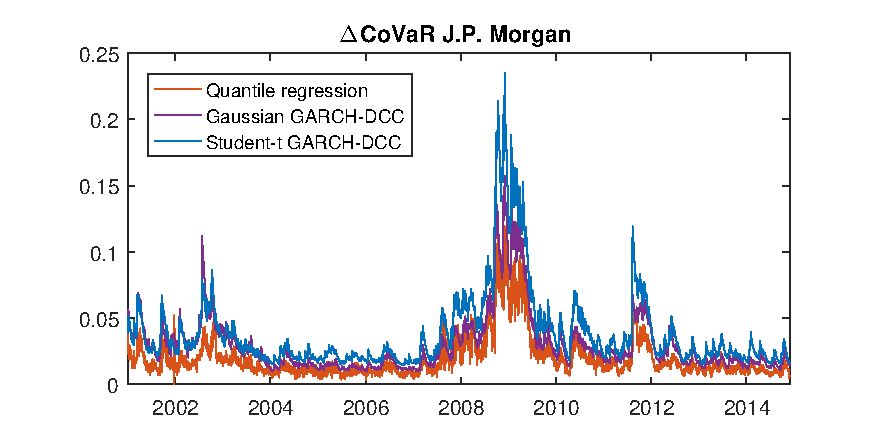
\includegraphics[width=1.1\textwidth]{Figure_5}}
\textit{\caption{ Estimated $\Delta CoVaR$ series for J.P. Morgan.  } \label{figr5}}
\end{figure}

\noindent In Figure \ref{figr5} the estimated $\Delta CoVaR$ series are shown for J.P. Morgan. The credit crisis of 2008 is clearly visible.

In the quantile regression, the dependency of the $CoVaR$ of $i$ on the return loss of $j$, captured by the parameter $\hat{\beta}_q$ in (\ref{eqcovq3}), does not change over time. In contrast, the Asymmetric GARCH-DCC model allows for time-varying correlation between the returns of $i$ and $j$. This is likely to be one of the reasons why the Asymmetric GARCH-DCC model outperforms the quantile regression. If, for example, the correlation between $X^i_t$ and $X^j_t$ increases over time, then $\hat{\beta}_q$ will underestimate the dependency and therefore, $x^j_t$ will have significant explanatory power on the occurrence of hits.

Table \ref{t445} also shows that for the 95\% $CoVaR$, the model using Gaussian innovations and the model using Student-$t$ innovations perform approximately equally well.  However, for the 99\% $CoVaR$, the Student-$t$ model clearly outperforms the Gaussian model. This is in line with our expectations since it is assumed that stock return distributions have heavier tails than the Gaussian distribution, in particular in the end of the tails \citep[e.g.,][]{bradley}.


%%% 26 CONCLUSION %%%


\section{Conclusion}


In this paper a new method for backtesting $Quantile$ $CoVaR$ predictions is introduced. Instead of testing the subset of $Tail$ $CoVaR$ predictions where the condition is satisfied (the approach used in previous research), we predict the $Q$-$CoVaR$ as a function of its condition (the return of $j$) and evaluate the predicted $Q$-$CoVaR$ at the realisation of this condition (the observed return of $j$). This allows us to perform tests on the full set of $Q$-$CoVaR$ predictions.

By definition, the observed return of $j$ should have no additional explanatory power on the hit series of a correctly specified $Q$-$CoVaR$ evaluated at the at the observed return of $j$. We include this property in the tests, which allows us to test whether there is misspecification in the dependency structure.

The Monte Carlo simulation shows that our test is useful in a realistic setting when we want to test whether a $CoVaR$ prediction method is specified correctly. It can detect both a distributional and a dynamic misspecification. Our test also outperforms previous $CoVaR$ backtesting methods in our simulation. The test is a little over-sized which is partly caused by the parameter estimation error. In line with \citet{nonlineartest}, we find that the linear test and the logistic test have a similar performance.

We predicted $Q$-$CoVaR$ series for the five largest US banks, where we used the Dow Jones US Financials Index as a proxy for the financial system.  We applied our tests to compare the performance of the quantile regression, the Asymmetric GARCH-DCC model with Gaussian innovations, and the Asymmetric GARCH-DCC model with Student-$t$ innovations.

The results indicate that the Asymmetric GARCH-DCC model with Student-$t$ innovations has the best ability to describe the underlying dynamics and that the quantile regression has the worst performance (out of the three estimation methods). A plausible explanation is that in the quantile regression, the dependency coefficient is fixed over time, while the Asymmetric GARCH-DCC model allows for time-varying correlation.

We also observe that the Student-$t$ innovations are outperforming the Gaussian innovations in particular in the end of the tail (i.e. the 99\% $CoVaR$). This may be due to the fatter tails of the Student-$t$ distribution.

Even if one prefers to use $T$-$CoVaR$ (based on an inequality condition) for a certain application (e.g. because of its monotonicity in the dependence parameter), our test might still be useful. One approach could be to first predict the $Q$-$CoVaR$ using different models and to apply our tests to find which model has the best performance. Then, using the preferred model, the $T$-$CoVaR$ can be predicted. This does not necessarily result in the optimal $T$-$CoVaR$ predictions. However, it may give better finite sample results than testing only a small subset of the $T$-$CoVaR$ predictions directly.

\citet{bayesian} apply Bayesian updating to the quantile regression coefficients to enable them to describe the time-varying dependency. An interesting approach for future research would be to use their prediction methods and to apply our tests to the Bayesian $Q$-$CoVaR$ predictions.

In this paper we focussed on the conditioning direction ``$VaR$ of the financial system given the return loss of $j$" ($CoVaR^{system|j}$). However, our test is equally applicable to the opposite definition where the $CoVaR$ is defined as the $VaR$ of an institution given that the financial system is in distress ($CoVaR^{i|system}$). This is also called ``\textit{Stressed Value at Risk}". Banks are required to calculate a $Stressed$ $VaR$ by the Basel II regulations. The $Stressed$ $VaR$ should be based on 10-day ahead predictions of the 99\% quantile \citep[][p. 14]{baselii}. Therefore, it would be an interesting approach for future research to investigate the performance of our test for 10-day ahead predictions.





\bibliographystyle{agsm}

\bibliography{Bibliography-MM-MC}
\end{document}

